\documentclass[11pt]{amsart}
\usepackage{geometry}                % See geometry.pdf to learn the layout options. There are lots.
\geometry{letterpaper}                   % ... or a4paper or a5paper or ... 
%\geometry{landscape}                % Activate for for rotated page geometry
%\usepackage[parfill]{parskip}    % Activate to begin paragraphs with an empty line rather than an indent
\usepackage{graphicx}
\usepackage{amssymb}
\usepackage{epstopdf}
\usepackage{setspace}
\onehalfspacing
%\usepackage{natbib}
\usepackage[authoryear,round]{natbib}
\usepackage{amsmath}
\newtheorem{theorem}{Theorem}[section]
\newtheorem{corollary}{Corollary}[theorem]
\newtheorem{lemma}[theorem]{Lemma}
\usepackage{amsthm}
 
\theoremstyle{definition}
\newtheorem{definition}{Definition}[section]
 
\theoremstyle{remark}
\newtheorem*{remark}{Remark}
\DeclareGraphicsRule{.tif}{png}{.png}{`convert #1 `dirname #1`/`basename #1 .tif`.png}

\title{Optimal design for nonlinear models with extension in T-sys}
\author{Yi Hua}
%\date{}                                           % Activate to display a given date or no date

\numberwithin{equation}{section}
\begin{document}

\maketitle

\section{Introduction}

Experiments are indispensable parts of scientific discovery and have broad application in industries including manufacture and pharmacy. People obtain insight into the cause-and-effect through logical analysis of appropriately designed experiments. However, as resources are limited, "good" experiments are always in demand to collect the most information for the given cost. In answer to this need, Optimal Designs addresses optimality with respect to some statistical criteria. When optimum estimation efficiency is of interest, we can use criteria based on the Fisher information matrix.

% An approximate design $\xi$ is comprised of the support points $x_i$'s and the corresponding weights $w_i$'s. An optimal design seeks the best choice of $\xi = \{(x_i,w_i), i=1,\ldots,n\}$ that maximizes the optimality criterion given a model. 

There have been extensive discussions on globally optimal designs for linear models. However, for nonlinear models, the information matrices depend on the unknown model parameters. As a result, the choice of an optimal design $\xi$ relies on presumed values of parameters and we can only determine locally optimal designs through numerical search. More importantly, since there is no canonical form for nonlinear models, the complexity and variety make the derivation and the numerical search a case-by-case situation. Many results based on the geometric approach by \cite{elfving1952} or equivalence theorem by \cite{kiefer1960} are available, but they are not transferable when new models or new objectives emerge. 

In answer to the challenges of identifying optimal designs for nonlinear models, \cite{dette2006}, \cite{yang2009}, \cite{yang2010}, \cite{dette2011}, \cite{yang2012}, and \cite{dette2013} provided a unified strategy that characterizes the optimal designs through complete class. Since determining the number of support points, $n$ is a critical step to identify optimal designs, to identify a complete class of designs of $n$ support points would largely reduce the complexity of numerical search and mathematical derivation. The strategy is to identify a subclass such that for any design $\xi$, there exists a design $\xi^*$ in the subclass, and $\xi^*$ dominates $\xi$ in terms of Lowener Ordeing. Consequently, we can focus on the subclass where we can search for $\xi^*$, which is our desired optimal design.
% To make this approach work, the subclass should be as simple as possible.


%  Biedermann, et al. (2006) provided s geometric solution of the number and locations of the support points of $\Phi_p$-optimal design.
 


%  In the manufacturing industry, experiments on performances of different designs need various expensive prototype products each being a support point. In that case, we want a minimal number of support points since making several products of the same prototype cost much less than more prototypes. In any scenario like this, we seek the design with a minimal number of support points among all optimal designs. 
 However, the assumptions required in the current strategy restrict the type of models it applies to. In this paper, we extended the method of \cite{yang2009}, \cite{yang2010}, and \cite{yang2012} to most nonlinear models using a tool called ancillary functions. We also showed that although involving ancillary functions seems increasing the number of support points needed, under certain conditions, we can remove the extra points. As a result, we could still obtain a minimally supported locally optimal design. We also demonstrated our method with the Beta-Poisson model, Skewed-logit model, and Complementary log-log model. The extended strategy can be readily applied to various dose-response models in clinical trials and nonlinear models in data science experiments to characterize optimal design with minimal support. 
%  For observational studies with a vast number of observations that is computationally expensive to fit model, the optimal design idea can be applied in sub-sampling of the observations to find the most informative points. Wang, Yang and Stufken (2018)\cite{iboss} has shown results in this scenario. 


In Section 2, we will discuss the model setup. In Section 3, we will introduce the current methodology and limitations. We will present our main results in Section 4 and further discussion in Section 5. 



\section{Model and Approximate Design}
Consider a nonlinear regression model $ E(y) = \eta(x,\theta)$, where a response variable $y$ depends on a single regression variable $x$. Assume $y$'s are independent and follow Bernoulli distribution with mean  $\eta(x,\theta)$. In the Design of Experiment scenario, the regression variable $x$ corresponds to a design point. The collection of design points and the weights $\xi = \{(x_i,w_i), i=\ldots,n\}$, $\sum_{i=1}^nw_i = 1$, $w_i> 0$ is called an approximate design. In many cases,  instead of $x_i$, it is more convenient to use $z_i$ which is a monotone,continuous function of $x_i$. For the rest of the paper, we will use $\xi = \{(z_i,w_i), i=\ldots,n\}$, $\sum_{i=1}^nw_i = 1$ as our goal. 

The goal of optimal design is to seek optimal choice of $\xi$ through characteristic of the fisher information matrix, which can be written as \begin{equation}\label{eq:1}
M(\xi,\theta) = \frac{\frac{\partial\eta(x,\theta)}{\partial\theta}(\frac{\partial\eta(x,\theta)}{\partial\theta})^T}{\eta(x,\theta)(1-\eta(x,\theta))} = P(\theta)(\sum_{i=1}^Nw_iC(\theta,z_i))P(\theta)^T
\end{equation}where \begin{equation}\label{eq:2}
C(\theta,z_i) = \left ( \begin{array}{cccc}
\Psi_{11}(z_i) &&&\\
\Psi_{21}(z_i) &\Psi_{22}(z_i)&&\\
\vdots & \vdots &&\\
\Psi_{p1}(z_i) &\Psi_{p2}(z_i)&\cdots&\Psi_{pp}(z_i)\\
\end{array} \right).\end{equation}
Due to the complexity of nonlinear models, the function $\Psi_{m,n}(\theta,z), m,n=1,\ldots,p$, and $M(\xi,\theta)$ may depend on $\theta$. Here for simplicity in notation, we will use $  \Psi_{m,n}(z)$ and $M(\xi)$. In \eqref{eq:1} and \eqref{eq:2}, $P(\theta)$ is independent of $x$ and $C(\theta,z)$ is symmetric. An optimal design $\xi = \{(z_i,w_i), i=\ldots,n\}$ maximizes the characteristic of  $M(\xi,\theta)$. For example, D-optimality uses $det(M(\xi,\theta))$ and A-optimality uses  $trace(M(\xi,\theta))$. 

In the mathematical derivation and numerical search of $\xi = \{(z_i,w_i), i=\ldots,n\}$ in the design space, a critical step is to determine the number of support points $n$. We can define a subclass of designs with $n$ support points such that for any design $\xi$, there exists a design $\tilde{\xi} = \{(\tilde{z_i},\tilde{w_i}), i=1,\ldots,N\}$ in the subclass that dominates $\xi$ in terms of Lowener Ordering as follows
\begin{equation}\label{l-ordering}
    M(\xi)\le M(\tilde{\xi}).
\end{equation} Here the inequality means $M(\tilde{\xi})-M(\xi)$ is a non-negative definite matrix.

To achieve this goal, \cite{yang2010} has introduced a sufficient condition of \eqref{l-ordering}: For $M(\xi)$ and $M(\tilde{\xi)}$ as defined in \eqref{eq:1} and \eqref{eq:2}, if 
\begin{equation}\label{eq: strategy1}
\sum_{i=1}^{n} w_i \Psi_{lt}(z_i) =\sum_{i=1}^{N} \tilde{w_i} \Psi_{lt}(\tilde{z_i}),\end{equation} for $1\le l\le t \le p$ except for some $l=t $, and, \begin{equation}\label{eq: strategy2}
\sum_{i=1}^{n} w_i \Psi_{ll}(z_i) \le \sum_{i=1}^{N} \tilde{w_i} \Psi_{ll}(\tilde{z_i}), \end{equation} are satisfied, the Loewner Ordering \eqref{l-ordering} is satisfied.
We can use \eqref{eq: strategy1} and \eqref{eq: strategy2} to find the complete class of designs with $n$ support points that contain the optimal design.


\section{Methodology and limitations} 
To identify the complete class of designs with $n$ support points, \cite{yang2012} and \cite{dette2011} used Tchebycheff System (abbreviated "T-system") as a bridge towards Lowener Ordering. The definition of a T-system is as follows.

\begin{definition}\label{deft}
    Let $u_0, \ldots, u_n$ denote continuous real-valued functions defined on a closed finite interval $[a,b]$, these functions will be called a \textbf{T-system} over $[a,b]$ provided  
\[U(u_0,\ldots,u_n, t_0,\ldots,t_n) = det\left ( \begin{array}{cccc}\label{eq: tdef2}
u_0(t_0) &u_0(t_1) &\ldots &u_0(t_n) \\
u_1(t_0) &u_1(t_1) &\ldots &u_1(t_n) \\
\vdots & \vdots &&\vdots\\
u_n(t_0) &u_n(t_1) &\ldots &u_n(t_n) \\
\end{array}\right)
    \] are strictly positive whenever $a\le t_0 <t_1< \ldots< t_n\le b$.
\end{definition}
% From the definition of a T-system , we can see that at least one of $\{\Psi_0(z),\Psi_1(z),\ldots, \Psi_k(z)\}$ and $\{\Psi_0(z),\Psi_1(z),\ldots, -\Psi_k(z)\}$ being T-systems on $[A,B]$ is a sufficient condition of Equation~\eqref{eq: tdef1} or Equation~\eqref{eq: tdef2}.

% On the other hand, since our target $\xi$ and $\tilde{\xi}$ are both designs, we have $\sum_i^nw_i = \sum_{i=1}^{k+1}\tilde{w}_i=1$. Here we will write $\tilde{w}_{k+1} = 1-\sum_{i=0}^{k} \tilde{w}_i$ and as a result, we also need to make sure $(\tilde{w}_1,\ldots, \tilde{w}_k)$ have unique solution. It's clear to see that, other than \eqref{eq: tsys1}, we also need to secure the following "smaller" system of equations to be consistent.
% \begin{equation}\label{eq: tsys2}
% \left ( \begin{array}{cccc}

% \Psi_{0}(\tilde{z}_1) &\Psi_{0}(\tilde{z}_2)&\ldots &\Psi_{0}(\tilde{z}_{k})\\
% \Psi_{1}(\tilde{z}_1) &\Psi_{1}(\tilde{z}_2)&\ldots &\Psi_{1}(\tilde{z}_{k})\\
% \vdots & \vdots &&\vdots\\
% \Psi_{k-1}(\tilde{z}_1) &\Psi_{k-1}(\tilde{z}_2)&\ldots &\Psi_{k-1}(\tilde{z}_{k})\\


% \end{array}\right) \left(\begin{array}{c}
%   \tilde{w}_1    \\
%   \tilde{w}_2    \\
%   \vdots\\
%     \tilde{w}_{k}    \\
      
% \end{array}\right) = \left(\begin{array}{c}
%   m_0    \\
%   m_1    \\
%   \vdots\\
%     m_{k-1}   \\
      
% \end{array}\right) 
% \end{equation} where $m_l = \sum_{i}w_i\Psi_l(z_i)$ for $l=0,1,\ldots,k$. 
% In order for \eqref{eq: tsys2} to have unique solution, following the same rationale, it is sufficient to shown that $\{\Psi_0(z),\Psi_1(z),\ldots, \Psi_{k}(z)\}$ is a T-system.
\cite{yang2012} showed in Theorem~\ref{2012a} that, if some subset of functions $\{\Psi_0(z)$, $\Psi_1(z)$, $\ldots$, $\Psi_{k-1}(z)$, $\Psi_k(z)^Q\}$ defined through information matrix $C(\theta,z)$ form T-systems, we can identify a complete class of designs.

\begin{theorem}[\cite{yang2012}]\label{2012a}
For a regression model with a single regression variable $x$, suppose that the information matrix $C(\theta,z)$ can be written as in \eqref{eq:1} and \eqref{eq:2} for $z\in[A,B]$. Partitioning the information matrix and let $\Psi_1(z),\ldots,\Psi_{k-1}(z)$ to be the maximum set of linearly independent non-constant terms in $p-p_1$ columns of $C(\theta,z)$. The remaining columns of $C(\theta,z)$ are denoted as $C_{22}(z)$.  $\Psi^Q_{k}(z)$ is defined as \[\Psi_k^Q(z) = Q^TC_{22}(z)Q\] where $Q$ is a nonzero vector of dimension $p_1\times 1$. Here $\Psi_k(z)$ is one of  $\Psi_{ll}(z), 1\le l \le p$. $\Phi_0(z) = 1$.
Suppose that either \begin{equation}\label{eq: 3.5}
    \{\Psi_0(z),\Psi_1(z),\ldots, \Psi_{k-1}(z)\} \text{ and }  \{\Psi_0(z),\Psi_1(z),\ldots, \Psi_k(z)^Q\} \text{ form T-systems,}
\end{equation}or\begin{equation}\label{eq: 3.6}
    \{\Psi_0(z),\Psi_1(z),\ldots,\Psi_{k-1}(z)\} \text{ and }  \{\Psi_0(z),\Psi_1(z),\ldots, -\Psi_k(z)^Q\} \text{ form T-systems.}
\end{equation}
     Then the following results hold:
\begin{enumerate}
    \item [(a)] For $k=2n-1$, if \eqref{eq: 3.5} holds, the designs with at most $n$ support points, including $B$, form a complete class
    
      \item [(b)] For $k=2n-1$, if \eqref{eq: 3.6} holds, the designs with at most $n$ support points, including $A$, form a complete class
      \item [(c)] For $k=2n$, if \eqref{eq: 3.5} holds, the designs with at most $n+1$ support points, including both $A$ and $B$, form a complete class
      \item [(d)] For $k=2n$, if \eqref{eq: 3.6} holds, the designs with at most $n$ support points form a complete class
    
\end{enumerate}
\end{theorem}
Here $\{\Psi_0(z)$, $\Psi_1(z)$, $\ldots$,$\Psi_{k-1}(z)$, $\Psi_k(z)^Q\}$ form a T-system means that \[U(\Psi_0(z),\ldots,\Psi_k^Q(z), z_0,\ldots,z_k)\] are strictly positive whenever $A\le z_0 <z_1< \ldots< z_n\le B$. It is worth mentioning here that, by matrix algebra, the sign of matrix determinant is invariant to certain row operations. We can multiply each function in $\{\Psi_0(z)$, $\Psi_1(z)$, $\ldots$,$\Psi_{k-1}(z)$, $\Psi_k(z)^Q\}$ by a function $g(z)$ as long as $g(z)>0$ for all $z\in [A,B]$ and that wouldn't change the sign of $U(\Psi_0(z),\ldots,\Psi_k^Q(z), z_0,\ldots,z_k)$. Adding a multiple of one row to another does not change the sign as well. This means that we can work instead on linearly independent terms of $\{\Psi_0(z)$, $\Psi_1(z)$, $\ldots$, $\Psi_{k-1}(z)$, $\Psi_k(z)^Q\}$, which could be convenient in some models. However, if we switch the order of the functions in $\{\Psi_0(z)$, $\Psi_1(z)$, $\ldots$, $\Psi_{k-1}(z)$, $\Psi_k(z)^Q\}$, we will change the order of rows in the matrix, which might result in a change of sign for $U(\Psi_0(z),\ldots,\Psi_k^Q(z), z_0,\ldots,z_k)$. Therefore, we need to be cautious with the order of the functions in the application. 



 However, to show a sequence of functions to be a T-system could be complicated and direct proof is not feasible. To achieve that, in the line of work in \cite{yang2009}, \cite{yang2010}, and \cite{yang2012}, a tool was developed to provide a sufficient condition to T-system.

 For $\{\Psi_0(z)$, $\Psi_1(z)$, $\ldots$,$\Psi_{k-1}(z)$, $\Psi_k(z)^Q\}$ as defined in Theorem~\ref{2012a}, and define functions $f_{l,t}, 1\le t \le k$; $t\le l \le k$ as follows
\begin{equation}\label{eq: ff}
f_{l,t}(z) = \left \{ \begin{array}{ll}
\Psi_l'(z), & \text{if } t=1,l=1,...,k-1\\
C'_{22}(z), & \text{if } t=1,l=k\\
(\frac{f_{l,t-1}(z)}{f_{t-1,t-1}(z)})', & \text{if } 2\le t\le k, t\le l \le k.
\end{array}\right.
\end{equation}
and   $F(z) = \prod_{l=1}^k f_{l,l}(z)$. 

\cite{yang2012} showed that $F(z)$ being positive definite is a sufficient condition of \eqref{eq: 3.5}. Also, $-F(z)$ being positive definite is a sufficient condition of \eqref{eq: 3.6}. As a result, we are able to work with the property of $F(z)$ to identify a complete class. However, the sufficiency is based on three critical assumptions during construction of $f_{l,t}(z)$ and $F(z)$.
\begin{enumerate}
\item All functions $\Psi$ in the information matrix $C(\theta,z)$ are at least $k$th order differentiable on $(A,B)$.
\item For $1\le l\le k-1$, the functions $f_{l,l}(z)$ have no roots in $[A,B]$.
\item Either $F(z)$ or $-F(z)$ is positive definite for all $z\in [A,B]$.
\end{enumerate} 


% The main result of \cite{yang2012} is as below.

% \begin{theorem}\label{2012}
% For a regression model with a single regression variable $x$, let $z\in[A,B]$, $C(\theta,z)$, $\Psi_1,\ldots, \Psi_{k-1}$ and $\Psi_k^Q$ defined above. With $F(z) = \prod_{l=1}^k f_{l,l}(z)$, suppose all assumption satisfied above. Then the following complete class results hold:\begin{enumerate}
% \item[(a)] For $k = 2n-1$, if $F(z)>0$, the designs with at most $n$ support points, including B, form a complete class.
% \item[(b)] For $k = 2n-1$, if $-F(z)>0$, the designs with at most $n$ support points, including A, form a complete class.
% \item[(c)] For $k = 2n$, if $F(z)>0$, the designs with at most $n+1$ support points, including both A and B, form a complete class.
% \item[(d)] For $k = 2n$, if $F(z)>0$, the designs with at most $n$ support points form a complete class.
% \end{enumerate}
% \end{theorem}

 This strategy has been applied to many non-linear dose-response models such as logistic model, LINEXP model, and double-exponential regrowth model. However, there are some models that we are not able to work with. For example, a complementary log-log model has the following form. \[P(y=1|x) = 1-e^{-e^{z}}, z\in(-\infty,\infty)\] If we follow the procedure in Theorem~\ref{2012a}, we will have the function sequence \[\{1,g(z), zg(z),z^2g(z)\},\text{ where }g(z)=\frac{e^{2z}}{e^{e^z}-1}.\] With this sequence, we can further calculate $f_{l,l}(z)$ and $F(z)$ by definition above. However, using Mathematica, we find that $f_{1,1}(z) = g'(z)$ has a root at $z=0.4660$, and $F(z)$ has a root at $z=0.0491$. Therefore, Assumption (2) and (3) are violated. As a result, we need to work on three disjoint intervals of z, $(-\infty, 0.0491)$, $(0.0491, 0.4660)$, and $(0.4660,\infty)$ separately. Applying Theorem~\ref{2012a}, we can obtain the complete class for three intervals respectively, each with 2 support points. Since there is no symmetry existing among the three intervals, we are not able to combine them as did in \cite{yang2009} to 2-parameter logistic model. The current strategy needs to be extended to address this case.
%  Meanwhile, \cite{biedermann2006} showed that the $\Phi_p$-optimal design for complementary log-log model defined on $(-\infty,\infty)$ is supported on 2 points. 

%  apply condition (a) of Theorem~\ref{2012} when $F(z) >0$ $z\in (-\infty, 0.0491)$, and condition (b) when $F(z)<0$ for $z\in(0.0491, 0.4660)$ and $(0.4660,\infty)$ respectively.

 
%  Another example of this situation is the 2-paraemter logistic model which has formula $P(y=1|x,\theta) = \eta(x,\theta)= \frac{1}{e^{-\beta(x-\alpha)}+1}$ where we let $z = \beta(x-\alpha) \in (-\infty, \infty)$ . Following the procedures from \eqref{eq:1} and \eqref{eq:2} , the information matrix based on a design $\xi = \{(z_i,w_i), i=1,\ldots,N\}$ will have the following form: \begin{equation}
% M(\xi) = \sum_{i=1}^{k} w_i \frac{e^z_i}{(1+e^{z_i})^2}P \left( \begin{array}{cc}
% 1 & z_i\\
% z_i & z_i^2
% \end{array} \right) P^T,
% \end{equation} where \[P = \left( \begin{array}{cc}
% \beta & 0\\
% 0 & -\frac{1}{\beta}
% \end{array} \right).\] \\

% Our goal is to find a design $\tilde{\xi} = \{(\tilde{z_i},\tilde{w_i}), i=1,\ldots,n\}$ such that $M(\xi)$ is dominated by $M(\tilde{\xi})$ by Loewner Ordering. Let $\phi(z) = \frac{e^z}{(1+e^{z})^2}$. To achieve this goal, if we could have the off-diagonal terms of both matrices to be equal as follows,
% \begin{equation}\label{eq: beta_eq1}
% \sum_{i=1}^{N} w_i \phi(z_i) = \sum_{i=1}^{n} \tilde{w_i}  \phi(\tilde{z_i}) ,
% \end{equation}
% and
% \begin{equation}\label{eq: beta_eq2}
% \sum_{i=1}^{N} w_i  \phi(z_i)z_i = \sum_{i=1}^{n} \tilde{w_i} \phi(\tilde{z_i}) \tilde{z_i},
% \end{equation}
% then it is sufficient to show that 
% \begin{equation}\label{eq: beta_eq3}
% \sum_{i=1}^{N} w_i \phi(z_i)z_i^2 \le \sum_{i=1}^{n} \tilde{w_i}\phi(\tilde{z_i})\tilde{z_i}^2.
% \end{equation}.

% To find solutions to the equations, direct application of \ref{2012} will also run into problems. Following the procedure of \ref{2012a},we need to show \{$1$ ,$ \phi(z)$, $z\phi(z)$, and $z^2\phi(z)$\} is a T-system. Also $\phi(z)>0$ holds for all $z$, therefore we can divide each term by $\phi(z)$ and move $1/\phi(z)$ to the last position (the sign changed) without loss of generality. The sequence is then equivalent to $\Psi_0(z) = 1$ , $\Psi_1(z) = z$ , $\Psi_2(z) = z^2$ , $\Psi_3(z) = -1/\phi(z)$. Calculation of $f_{l,l}(z)$, $l=1,2,3$ shows that $f_{1,1}(z) = 1$, $f_{2,2}(z) = 2$, $f_{3,3}(z) = -3 (1 + e^z) + e^{-z} (1 + e^z)^2/2 + 
%  3 e^{-z} (2 e^{2 z} + 2 e^z (1 + e^z))/2 - 
%  e^{-z} (6 e^{2 z} + 2 e^z (1 + e^z))/2 $.  \[F(z) = -6 (1 + e^z) + e^{-z} (1 + e^z)^2 + 
%  3 e^{-z} (2 e^{2 z} + 2 e^z (1 + e^z)) - 
%  e^{-z} (6 e^{2 z} + 2 e^z (1 + e^z))\]
%  \begin{figure}[h]
%      \centering
%      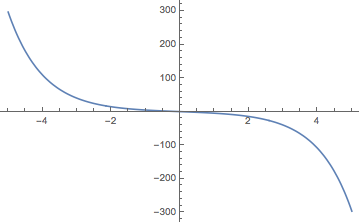
\includegraphics[scale = 0.5]{logistic.png}
%      \caption{$F(z)$ for 2-parameter logistic model}
%      \label{fig:logistic}
%  \end{figure}
%  Apparently, third assumption is not satisfied throughout $(-\infty,\infty)$ since $F(0)=0$, but we do get results for $(-\infty,0)$ and $(0,\infty)$ separately. Specifically for $z>0$, $F(z) <0$, and for $z<0$, $F(z) >0$. To get around this hurdle, we could apply \ref{2012} for $z\in[\epsilon, \infty)$ and $z\in(-\infty,-\epsilon]$, $\epsilon>0$,respectively. Here $k=3$. For $z\in[\epsilon, \infty)$, $\epsilon>0$, $F(z)<0$,  designs with 2 support points including $\epsilon$ form a complete class. For $z\in(-\infty,-\epsilon]$, $\epsilon>0$, $F(z)>0$,designs with 2 support points including $-\epsilon$ form a complete class. As $\epsilon\to 0$, the optimal design for each side of $0$ will be \{0,$x_1>0$\} and \{0,$x_2<0$\}. On the other hand Biederman (2006) was able to show that 2- parameter logistic regression defined on $(-\infty,\infty)$ has $\Phi_p$-optimal design with 2 support points.
 
%  We try to work with the function sequence \{$1$ ,$\phi(z)$, $z\phi(z)$, and $z^2\phi(z)$\} and insert some ancillary functions. Here we insert $1/(1+e^z)^2$ in front of $1$. We then are now working with equations 
 
% \begin{equation}\label{eq: log_eq1}
% \sum_{i=1}^{N} w_i \frac{1}{(1+e^{z_i})^2} = \sum_{i=1}^{n} \tilde{w_i}  \frac{1}{(1+e^{\tilde{z_i}})^2} ,
% \end{equation}

% \begin{equation}\label{eq: log_eq2}
% \sum_{i=1}^{N} w_i  = \sum_{i=1}^{n} \tilde{w_i}  ,
% \end{equation}

% \begin{equation}\label{eq: log_eq3}
% \sum_{i=1}^{N} w_i \phi(z_i) = \sum_{i=1}^{n} \tilde{w_i}  \phi(\tilde{z_i}) ,
% \end{equation}

% \begin{equation}\label{eq: log_eq4}
% \sum_{i=1}^{N} w_i  \phi(z_i)z_i = \sum_{i=1}^{n} \tilde{w_i} \phi(\tilde{z_i}) \tilde{z_i},
% \end{equation}

% \begin{equation}\label{eq: log_eq5}
% \sum_{i=1}^{N} w_i \phi(z_i)z_i^2 \le \sum_{i=1}^{n} \tilde{w_i}\phi(\tilde{z_i})\tilde{z_i}^2.
% \end{equation}.Note here that \ref{eq: log_eq2} is also inherent in \ref{eq: beta_eq1}-\ref{eq: beta_eq3} since $\xi$ and $\tilde{\xi}$ are both designs. Since we now have one extra \ref{eq: log_eq1} in the equation system \ref{eq: log_eq1}-\ref{eq: log_eq5} will have solutions that also satisfy \ref{eq: beta_eq1}-\ref{eq: beta_eq3}, but will most certainly include more $(\tilde{z_i},\tilde{w_i})$. In this sense, the insertion of some  "ancillary" functions will not affect the validity of the solution, although it may most likely include more support points than we desired.

% Now that we have a "bigger" design, we'll see how the ancillary functions may help with the violated assumptions. We are now working with \{$1/(1+e^z)^2$, $1$ ,$\phi(z)$, $z\phi(z)$, and $z^2\phi(z)$\}. We can do a similar trick of multiplying each function with $(1+e^z)^2>0$ , take linearly independent terms and check if  \{$1$, $e^{2z}$ ,$e^z$, $ze^z$, $z^2e^z$\} is a T-system. We then proceed to use \ref{2012} and have $f_{1,1}(z) = 2e^{2z}$, $f_{2,2}(z) = -e^{-z}/2$,$f_{3,3}(z) = 1$,$f_{4,4}(z) = 2$, and $f(z) = -2e^z<0$ for $z\in(-\infty,\infty)$. Now we can safely apply \ref{2012} on $[-A,B]$ for any  $A,B>0$. Luckily, we have that designs with at most 2 support points form a complete class. \\




%  In Yang (2009), the author managed to "combine" optimal designs of the two sides, using the fact that $\phi(z)$ is an even function, and there exists a complete class of 2 support-point design, in which the two points are symmetric about $0$. The author also managed to show the same strategy used in finding designs with two symmetric points for 2-parameter probit model. For double exponential and double reciprocal model, the author showed there exists a complete class of 3 support that contains 0 and two symmetric points. All results are based on the symmetry of the above models.
 


% We have now seen from the 2-parameter logistic model that use of ancillary functions ($1/(1+e^z)^2)$ helped solve the problem of assumption violation. We now formally introduce the use of ancillary functions for general models. 

\section{Main Results}
To extend the application of the strategy in \cite{yang2012} to more models, here we introduced the use of Ancillary Functions.  
\subsection{The Ancillary functions} 
\begin{definition}[Ancillary Functions]
    For nonlinear model $E(y) = \eta(x,\theta)$, let \[S_1 = \{\Psi_0(z), \Psi_1(z), \ldots,\Psi_{k-1}(z) ,\Psi_k^Q(z)\}\] be functions defined in Theorem~\ref{2012a}. Denote a set of functions \[ S_2 =\{\phi^*_1(z), \phi^*_2(z),\ldots, \phi^*_{k_1}(z)\}\] where $\phi^*_i(z)$, $i=1,\ldots,k_1$ are at least $k$th order differentiable.  Here functions in $S_2$ are mutually linearly independent and independent of functions in $S_1$. We call $S_2$ Ancillary Functions of $S_1$.
\end{definition}

 To use ancillary functions $S_2$, we insert functions in $S_2$ to $S_1$ before the last function $\Psi_k^Q(z)$. Let the order of the terms in $S_1$ remain unchanged. Denote the new sequence as  \[S_3 = \{\tilde{\Psi}_0(z), \tilde{\Psi}_1(z), \ldots,\tilde{\Psi}_{k+k_1-1}(z), \tilde{\Psi}_{k+k_1}^Q(z)\}.\] For a proper choice of $S_2$, working with $S_3$ instead of $S_1$ could avoid violation of assumptions. As mentioned of the current strategy in \eqref{eq: ff}, the calculation of $f_{l,l}(z)$ largely reply on the hierarchy of the functions, i.e., the orders and divergence rates of $\Psi_i(z)$'s. For non-symmetric models including complementary log-log model, the function sequence is not amenable to the assumptions. Here we introduce the ancillary functions to those models that do not have a "good tier" in $S_1$. Inserting $\phi_i^*(z)$'s in between the $\Psi_i(z)$'s will form a better organized sequence, which will not violate the assumptions. The details of application will be demonstrated in Section 4.3-4.5.

Rewriting our goal in \eqref{eq: strategy1} and \eqref{eq: strategy2} in terms of $S_1$, we have  
\begin{equation} \label{eq: st1}
\sum_{i}w_i\Psi_l(z_i)=\sum_{i}\tilde{w_i}\Psi_l(\tilde{z_i}), l=0,1,\ldots, k-1
\end{equation} and \begin{equation} \label{eq: st2}
\sum_{i}w_i\Psi_k^Q(z_i)<\sum_{i}\tilde{w_i}\Psi_k^Q(\tilde{z_i}) \text{  for every nonzero vector Q}
\end{equation}  
\begin{lemma}
Given $S_1$ and a properly defined ancillary function sequence $S_2$, use of the extended function sequence $S_3$ is sufficient to \eqref{eq: st1} and \eqref{eq: st2}
\end{lemma}
\begin{proof}
Consider the new sequence $S_3$ as the function sequence used in \eqref{eq: st1} and \eqref{eq: st2}, we will have \begin{equation}\label{eq: added1}
\sum_{i}w_i\Psi_l(z_i)=\sum_{i}\tilde{w_i}\Psi_l(\tilde{z_i}), l=0,1,\ldots, k-1    
\end{equation}
\begin{equation}\label{eq: added2}
\sum_{i}w_i\phi_j^*(z_i)=\sum_{i}\tilde{w_i}\phi_j^*(\tilde{z_i}), j=1,\ldots, k_1    
\end{equation}and \begin{equation}\label{eq: added3}
\sum_{i}w_i\Psi_k^Q(z_i)<\sum_{i}\tilde{w_i}\Psi_k^Q(\tilde{z_i}) \text{  for every nonzero vector Q}.
\end{equation} 
As \eqref{eq: st1} and \eqref{eq: st2} are included in the new system of equations, we will still obtain a design that satisfy \eqref{eq: st1} and \eqref{eq: st2}. Therefore, the function sequence $S_3$ with ancillary functions $S_2$ still leads to a complete class of designs that is "optimal" in Loewner Ordering. The new design could include more support points than desired, as there are more equations. We'll show in the following discussions that for some models, the "extra" points can actually be removed under certain circumstances.
\end{proof}


% Since all original $\Psi$ functions are from information matrix $C(\theta,z)$, the extended function sequence also suggests an "enlarged" information matrix $\tilde{C}(\theta,z)$. What we do is to add rows and columns to $C(\theta,z)$ and fill in the ancillary function symmetrically. Consider $k_1\le p+1$, we can write \begin{equation}
%   \tilde{C}(\theta,z) = \left ( \begin{array}{c|ccccc}
% \multicolumn{1}{c}{\phi^*_1}& \ldots& \phi^*_{k_1} &0 &\ldots& 0\\\cline{2-6}
% \vdots &  &&&&\\
% \phi^*_{k_1} &&&&&\\
% 0 &\multicolumn{5}{|c}{C(\theta,z)}\\
% \vdots &&&&&\\
% 0&&&&&
% \end{array}\right)_{(p+1)\times (p+1)}.
% \end{equation} 

% When $ p+1< k_1 \le2p+3$, we can write\begin{equation}
%   \tilde{C}(\theta,z) = \left ( \begin{array}{cc|ccccc}
% \phi^*_{p+2}& \multicolumn{1}{c}{\phi^*_{p+3}}&  \ldots& \phi^*_{k_1} &0 &\ldots& 0\\
% \phi^*_{p+3}&\multicolumn{1}{c}{\phi^*_{1}}& && \ldots&& \phi^*_{p+1}\\\cline{3-7}
% \vdots &  &&&&&\\
% \phi^*_{k_1} &&&&&\\
% 0 &\vdots &\multicolumn{5}{|c}{C(\theta,z)}\\
% \vdots &&&&&&\\
% 0&\phi^*_{p+1}&&&&&
% \end{array}\right)_{(p+2)\times (p+2)}.
% \end{equation} We can write $\tilde{C}(\theta,z)$ for larger $k_1$ following the same procedure if needed. However, since our goal is to obtain a design with minimal support, we usually expect $k_1$ to be small. We will discuss the details in next section. $\tilde{C}(\theta,z)$ will be the surrogate of $C(\theta,z)$ to apply \ref{2012}.



%\begin{theorem}(show that ancillary terms doesn't change inequality and how many more support points will be added according to the number of ancillary functions added)
%For nonlinear model $E(y) = \eta(x,\theta)$, let $\Psi_1, \ldots,\Psi_{k-1}$ and $\Psi_k^Q(z)$ be functions defined above. Add $\phi^*_1(z), \phi^*_2(z),\ldots, \phi^*_{k_1}(z)$ to the function sequence before  $\Psi_k^Q(z)$. Here  $\phi^*_1(z), \phi^*_2(z),\ldots, \phi^*_{k_1}(z)$ are mutually linearly independent and independent of   $\Psi_1, \ldots,\Psi_{k-1}$ and $\Psi_k^Q(z)$ (element-wise). Denote the new sequence as  \{$\tilde{\Psi_1}, \ldots,\tilde{\phi}_{k+k_1-1}, \tilde{\phi}_{k+k_1}^Q(z)$\}. Let $\tilde{\phi}_0(z) = 1$. \\

%If we have \begin{equation}\label{cheby+}\{\tilde{\phi}_0(z), \tilde{\phi}_1(z), \ldots,\tilde{\phi}_{k+k_1-1}(z)\}  \text{ and }  \{\tilde{\phi}_0(z), \tilde{\phi}_1(z), \ldots,\tilde{\phi}_{k+k_1-1}(z), \tilde{\phi}_{k+k_1}^Q(z)\}  \end{equation} form T-systems for every nonzero vector $Q$ or \begin{equation}\label{cheby-} \{\tilde{\phi}_0(z), \tilde{\phi}_1(z), \ldots,\tilde{\phi}_{k+k_1-1}(z)\}  \text{ and }   \{\tilde{\phi}_0(z), \tilde{\phi}_1(z), \ldots,\tilde{\phi}_{k+k_1-1}(z), -\tilde{\phi}_{k+k_1}^Q(z)\}  \end{equation}form T-systems for every nonzero vector $Q$.\\    \end{theorem}

 

%  The expanded $C(\theta,z)$ will be \[ \tilde{C}^*(\theta,z) = \phi(z)\left(\begin{array}{ccc}
% 1 &e^{2z}&0\\
% e^{2z}&e^z & ze^z\\
% 0& ze^z & z^2e^z
% \end{array} \right).\]Note now $k=4$. Calculate $f_{l,l}(z), l=1,\ldots, 4$, we have $f_{1,1}(z) = 2e^{2z}$, $f_{2,2}(z) = -e^{-z}/2$ , $f_{3,3}(z) = 1$, $f_{4,4}(z) = 2$. As s result $F(z)<0$ for $z\in (-\infty, \infty)$. We have condition (d) satisfied and the designs with at most 2 support points form a complete class. This result is consistent with the conclusion in Yang (2009). \\
 




% We have shown in the 2-parameter logistic model that our strategy can deal with the failed assumptions. Before getting to the details of ancillary functions, we will justify the extension to models defined on open interval first. In Yang (2010) and Yang 2012), the results all focused on models defined on closed intervals. The following result shows that we do not have the issue of "non-informative " support points with models defined on a closed interval. This is not the case when extended to open intervals. 

% \begin{lemma}(Models defined on $[A,B]$ cannot have an optimal design that includes support point $I(A)$ or $I(B) =0$)

% Suppose we have a nonlinear regression model defined on $[A, B]$. Information matrix are defined as \eqref{eq:1} and \eqref{eq:2}. Suppose there exist $z^*\in [A, B]$ such that $I(z^*)=0$, the optimal design decided by Loewner ordering will not include that point.
% \end{lemma}

 
 
\subsection{Removable Boundary Points}
The use of ancillary functions might require more support points than desired in the design, which could lead us to a complete class of designs with more support points. Here we show in the following results that, for some functions defined on an open interval, we can find a design in a complete class with fewer support points that dominates the "enlarged" design. In this sense, the added support points could be "removed" from the design. 

We use the following definition to classify nonlinear models regarding their properties on the boundary points. 
\begin{definition} We categorize models defined on $(A,B)$ into the following 4 types\begin{enumerate}
    \item Type I: $\lim_{z\to A}I(z)=0$ and $\lim_{z\to B}I(z)\ne 0$
    \item Type II: $\lim_{z\to A}I(z)\ne 0$ and $\lim_{z\to B}I(z)=0$
    \item Type III: $\lim_{z\to A}I(z)= 0$ and $\lim_{z\to B}I(z)=0$
    \item Type IV: $\lim_{z\to A}I(z)\ne 0$ and $\lim_{z\to B}I(z)\ne0$
\end{enumerate}
\end{definition}

% \begin{lemma} For nonlinear models with response $E(Y) = \eta(\theta,z)$, $z\in (A,B)$. If there exist $z^*\in [A,B]$ such that \[\lim_{z\to z^*}(\frac{\partial\eta(\theta,z)}{\partial \theta}) = 0\]
% then $\lim_{z\to z^*}I(\theta,z)=0$
% \begin{proof}
% Binary response
% \[\lim_{z\to z^*}I(\theta,z) = \lim_{z\to z^*}\frac{(\frac{\partial\eta(\theta,z)}{\partial \theta})(\frac{\partial\eta(\theta,z)}{\partial \theta})^T}{\eta(\theta,z)(1-\eta(\theta,z))} = 0\]


% %  Continuous response
% %  \[\lim_{z\to z^*}I(\theta,z) = \lim_{z\to z^*}(\frac{\partial\eta(\theta,z)}{\partial \theta})(\frac{\partial\eta(\theta,z)}{\partial \theta})^T = 0\]
%  \end{proof}
%  \end{lemma}

\begin{theorem}\label{removepts}
 Suppose we have a non-linear model with a single regression variable $z$ defined on $(A,B)$. Consider any subset $[A^*,B^*]\subset (A,B)$, on which we were able to identify a complete class of designs with $n$ support points through Theorem~\ref{2012a}. Here $A^* = A+\epsilon$ and  $B^* = B-\epsilon$ for some small $\epsilon>0$. Denote the optimal design in the complete class as $\xi$ = \{$(z_1,w_1)$, $(z_2,w_2)$, $\ldots$, $(z_n,w_n)$\} where $A<A^*\le z_1< \ldots< z_n \le B^*<B$. We have the following results.\begin{enumerate}
     
     \item If the model is of Type I, and $z_1=A^*$, then $\xi$ is dominated by $\xi^*$ = \{$(z_2,w_1+w_2)$, $(z_3,w_3)$, $\ldots$, $(z_n,w_n)$\} where $A^* < z_2 <\ldots< z_n\le B^*$, as $\epsilon\to 0$.  $\xi^*$ belongs to a complete class of designs with $n-1$ support points.
     \item If the model is of Type II, and $z_n=B^*$, then $\xi$ is dominated by $\xi^*$ = \{$(z_1,w_1)$, $(z_2,w_2)$, $\ldots$, $(z_{n-1},w_{n-1}+w_n)$\} where $A^*\le z_1 <\ldots< z_{n-1}< B^*$, as $\epsilon\to 0$.  $\xi^*$ belongs to a complete class of designs with $n-1$ support points.
     \item If the model is of Type III, $z_1 = A^*$, and $z_n=B^*$, then $\xi$ is dominated by $\xi^*$ = \{$(z_2,w_2+w_1)$, $(z_3,w_3)$, $\ldots$, $(z_{n-2},w_{n-2})$,  $(z_{n-1},w_{n-1}+w_n)$\} where $A^*< z_2 <\ldots< z_{n-1}< B^*$, as $\epsilon\to 0$.  $\xi^*$ belongs to a complete class of designs with $n-2$ support points.
     \item If the model is of Type III, $z_1 = A^*$, and $z_n<B^*$, then $\xi$ is dominated by $\xi^*$ = \{$(z_2,w_1+w_2)$, $(z_3,w_3)$, $\ldots$, $(z_n,w_n)$\} where $A^* < z_2 <\ldots< z_n< B^*$, as $\epsilon\to 0$.  $\xi^*$ belongs to a complete class of designs with $n-1$ support points.
     \item If the model is of Type III, $z_1 > A^*$, and $z_n = B^*$, then $\xi$ is dominated by $\xi^*$ = \{$(z_1,w_1+w_n)$, $(z_2,w_2)$, $\ldots$, $(z_{n-1},w_{n-1})$\} where $A^*< z_1 <\ldots< z_{n-1}< B^*$, as $\epsilon\to 0$. $\xi^*$ belongs to a complete class of designs with $n-1$ support points.
     
     \item In all other cases, we cannot find a design $\xi^*$ from a different complete class that dominates $\xi$.
 \end{enumerate}
\end{theorem}

From Theorem~\ref{removepts}, we can see that it is possible for us to reduce the support for certain types of model. With this tool,  we can cut the enlarged design with ancillary functions back to minimal support. 

  

 

% We now are able to extend the conclusion in \ref{2012} to models defined on open interval $(A,B)$ under following assumptions. \begin{enumerate}
% \item All functions $\Psi$ in the information matrix $C(\theta,z)$ are at least $k$th order differentiable on $(A,B)$.
% \item For $1\le l\le k-1$, the functions $f_{l,l}(z)$ have no roots in $(A,B)$.
% \end{enumerate} 


% \begin{theorem}\label{2012open}
% For a regression model with a single regression variable $x$, let $z\in(A,B)$, $C(\theta,z)$, $\Psi_1,\ldots, \Psi_{k-1}$ and $\Psi_k^Q$ defined above. With  $F(z) = \prod_{l=1}^k f_{l,l}(z)$, suppose that either $F(z)$ or $-F(z)$ is positive definite for all $z\in (A,B)$. Then the following complete class results hold:\begin{enumerate}
% \item[(a)] For $k= 2n-1$, if Type II or Type III models have $F(z)>0$,  designs with at most $n-1$ support points form a complete class; if Type I or Type IV models have $F(z)>0$,  designs with at most $n$ support points form a complete class. 
% \item[(b)] For $k= 2n-1$, if Type I or Type III models have $-F(z)>0$,  designs with at most $n-1$ support points form a complete class; if Type II or Type IV models have $-F(z)>0$,  designs with at most $n$ support points form a complete class. 
% \item[(c)] For $k = 2n$, if Type III model have $F(z)>0$, designs with at most $n-1$ support points form a complete class; if Type I or Type II model have $F(z)>0$, designs with at most $n$ support points form a complete class; if Type IV model have $F(z)>0$, designs with at most $n+1$ support points form a complete class
% \item[(d)] For $k = 2n$, if models of any type have $-F(z)>0$, designs with at most $n$ support points form a complete class.
% \end{enumerate}
% \end{theorem}
% \begin{proof} 
% The proof is similar for the four conditions. We will here show for (a)  \\
% By \ref{2012}, if $k = 2n-1$ and $F(z)>0$, design with at most n support points form a complete class. Consider for any design $\xi = \{z_1,z_2,\ldots, z_n\}$, there exist $\tilde{\xi} = \{\tilde{z}_1,\tilde{z}_2,\ldots, \tilde{z}_{n-1}, B-\epsilon\}$, $\epsilon>0$ such that \[M(\xi)\le M(\tilde{\xi}) =\sum_i^{n-1} \tilde{w}_iI(\tilde{z}_i)+\tilde{w}_nI(B-\epsilon) \] 
% Since for Type II or Type III models,  $\lim_{z\to B}I(z)=0$, we have zero information at $B$. Without loss of generality, we could assign $w_n$ to $\tilde{z_1}$, which lead to a design $\{(\tilde{z}_1, \tilde{w}_1+\tilde{w}_n), (\tilde{z}_2, \tilde{w}_2),\ldots,(\tilde{z}_{n-1}, \tilde{w}_{n-1}) \}$. This design has $n-1$ support points. 
% For Type II or Type III models, $\lim_{z\to B}I(z)\ne0$ so we are not able to eliminate this point from design. The design with $n$ support points form a complete class.
% \end{proof}




% With \ref{2012open}, we can deal with models defined on open interval and eliminate the boundary points that provide 0 information asymptotically. \\

% The next issue to address is the resolution to failed assumptions. In the example of the 2-parameter logistic model, the ancillary function enables us to use \ref{2012} with minimal support. In many other cases, the aid of ancillary functions will work at the price of getting a design with more support points. Below is a tentative strategy for choosing ancillary function  %The validity of ancillary functions is also shown. Suppose we already have the ancillary functions and $\tilde{F}(z)>0$ or $-\tilde{F}(z)>0$ 


% \begin{theorem}(how many ancillary functions to use/ where to insert)For a given model with predictor variable $z$ and information matrix at a point $z$ $I(z)$, $z\in[A,B]$, suppose the assumption of \ref{2012} is violated for a function sequence $\{\Psi_0(z),\Psi_1(z),\ldots, \Psi_k(z)\}$, we can insert $k_1$ ancillary functions into the sequence so that the number of support point remain the same. The strategy is as follows, \begin{enumerate}
%     \item If $\lim_{z\to A}I(z)=0$, choose $k_1\le 3$ such that $k+k_1 = 2n-1$ , change the position of insertion so that $-F(z)>0$ for all $z\in [A,B]$.
%     \item If $\lim_{z\to B}I(z)=0$, choose $k_1\le 3$ such that $k+k_1 = 2n-1$ , change the position of insertion so that $F(z)>0$ for all $z\in [A,B]$.
%     \item If $\lim_{z\to A}I(z)=0$ and $\lim_{z\to B}I(z)=0$ , choose $k_1\le 3$ such that $k+k_1 = 2n$, change the position of insertion so that $F(z)>0$ for all $z\in [A,B]$.
%     \item If $\lim_{z\to A}I(z)\ne 0$ and $\lim_{z\to B}I(z)\ne 0$ , choose $k_1\le 3$ such that $k+k_1 = 2n$, change the position of insertion so that $-F(z)>0$ for all $z\in [A,B]$.
% \end{enumerate}

% \end{theorem}



% \begin{corollary}(Closed interval, assumptions failed)
% For a regression model with a single regression variable $x$, let  $z\in[A,B]$, $C(\theta,z)$, $\Psi_1(z), \ldots,\Psi_{k-1}(z)$ and $\Psi_k^Q(z)$ be as in \ref{2012}. Assume all functions $\Psi_i(z)$, $i=1,..,k$ are at least $k$th order differentiable on $(A,B)$ element-wise. Also assume there exist at least one $l_0$, $1\le l_0\le k-1$, and $z^*\in [A,B]$, such that $f_{l_0,l_0}(z^*) = 0 $. Use $k_1$ ancillary functions to extend the function sequence to \{$\tilde{\Psi}_1(z), \ldots,\tilde{\Psi}_{k+k_1-1}(z), \tilde{\Psi}_{k+k_1}^Q(z)$\} as in \ref{proc}. Assume $\tilde{F}(z) = \prod_{l=1}^{k_1+k}\tilde{f}_{l,l}(z)$ with the new sequence. Suppose that either $\tilde{F}(z)$ or $-\tilde{F}(z)$ is positive definite for all $z\in [A,B]$. The following complete class results hold \begin{enumerate}
% \item[(a)] For $k+k_1= 2n-1$, if $\tilde{F}(z)>0$,  designs with at most $n$ support points, including B, form a complete class. 
% \item[(b)] For $k+k_1= 2n-1$, if $-\tilde{F}(z)>0$,  designs with at most $n$ support points, including A, form a complete class.
% \item[(c)] For $k+k_1 = 2n$, if $\tilde{F}(z)>0$,  designs with at most $n+1$ support points, including A and B, form a complete class.
% \item[(d)] For $k+k_1 = 2n$, if $-\tilde{F}(z)>0$,  designs with at most $n$ support points form a complete class.

% \end{enumerate} 

% \end{corollary}


% Through the above results, we can see nonlinear models that failed assumptions can use ancillary functions to find optimal design at the cost of including extra support on the boundary. Among these models, Type I, II and III models under certain conditions may enable us to remove the extra support points and achieve minimal support. We will demonstrate the combination of two main results in the next section.


% The following is a tentative procedure of which may be helpful for finding the ancillary functions. We will demonstrate with examples of how this procedure is used in the next section.

% \begin{theorem}\label{proc}(How to insert ancillary functions: still working)
% Given a nonlinear model, suppose for a function sequence $S_1 = \{\Psi_l(z), l = 1,\ldots,k\}$, neither $F(z)$ or $-F(z)$ is positive definite, we can use the following steps to insert ancillary functions to the sequence. Let $S = S_1$.
% \begin{enumerate}
%     \item Select a function $\phi(z)$ that is the common factor of most $\Psi$ functions. Choose another one if it is linearly dependent to functions in $S$. If $1\not\in S$, let $\phi(z) = 1$. Update $S = S\cup\{\phi(z)\}$. Update $\tilde{C}(\theta,z)$ with $S$.
%     \item Multiply each term of $S$ by least common multiples of the denominators, if any. Update $\tilde{C}(\theta,z)$ 
%     \item Take Minimal common factors of the sequence. Start from adding factors shared among most $\Psi$ functions. It will , after matrix algebra, be placed before the lowest order term that contains that factor. Check $F(z)$, if not satisfying the assumptions continue until run out of factors.
    
%     \item Clean up the functions so that they are linearly independent, leaving the terms of highest order as is. Update $S = {S,\phi(z)}$. Update $\tilde{C}(\theta,z)$ with $S$.
%      \item Calculate $\tilde{F}(z)$. Check if $\tilde{F}(z)$ or $-\tilde{F}(z)$ is positive definite. Record $k_1$ as the number of functions added. If not, repeat 1-3.
% \end{enumerate}
% \end{theorem}



\subsection{Beta-Poisson model}

In  studies of binary dose response relationship, Beta-Poisson model is an important model. The response $y$ follows a Bernoulli distribution with the expected success probability of the following form
\[
P(y=1|x,\theta_1,\theta_2) = \eta(x,\theta_1,\theta_2)= 1-(1+\frac{x}{\theta_2})^{-\theta_1}.
\]
 Here $x> 0$ is dose level, with $\theta_1>0$ being the infectivity and $\theta_2>0$ being the shape parameter. Let $z = log(1+\frac{x}{\theta_2})$, and we know $z>0$. Consider range of $z$ to be $(0,+\infty)$. Denote $\theta = (\theta_1,\theta_2)$. Simple calculation shows that it is a Type I model. The information matrix based on a design $\xi = \{(z_i,w_i), i=1,\ldots,N\}$ will have the following form: \begin{equation}
M(\xi) = \sum_{i=1}^{k} w_iP C(\theta,z_i)P^T 
\end{equation} where \begin{align*}
    P &= \left( \begin{array}{cc}
1 & 0\\
0 & -\frac{\theta_1}{\theta_2}
\end{array} \right), \text{and}\\ 
C(\theta,z_i) &= \frac{e^{-\theta_1z_i}}{1-e^{-\theta_1z_i}}\left( \begin{array}{cc}
z_i^2 & z_i(1-e^{-z_i})\\
z_i(1-e^{-z_i}) & (1-e^{-z_i})^2
\end{array} \right).
\end{align*} 

Our goal is to identify a complete class that contains a design $\tilde{\xi} = \{(\tilde{z_i},\tilde{w_i}), i=1,\ldots,n\}$ such that \[M(\tilde{\xi})-M(\xi)>0.\] Let $g(z) = \frac{e^{-\theta_1z}}{1-e^{-\theta_1z}}$. To achieve this goal, if we could have the off-diagonal terms of both matrices to be equal as follows,
\begin{equation}\label{eq: beta2_eq1}
\sum_{i=1}^{N} w_i g(z_i)z_i(1-e^{-z_i}) = \sum_{i=1}^{n} \tilde{w_i}  g(\tilde{z_i}) \tilde{z_i}(1-e^{-\tilde{z_i}}),
\end{equation}
then it is sufficient to show that 
\begin{equation}\label{eq: beta2_eq2}
\sum_{i=1}^{N} w_i  g(z_i)(1-e^{-z_i})^2 \le \sum_{i=1}^{n} \tilde{w_i} g(\tilde{z_i}) (1-e^{-\tilde{z_i}})^2,
\end{equation}
and
\begin{equation}\label{eq: beta2_eq3}
\sum_{i=1}^{N} w_i g(z_i)z_i^2 \le \sum_{i=1}^{n} \tilde{w_i}g(\tilde{z_i})\tilde{z_i}^2.
\end{equation} 
% where equality in \eqref{eq: beta2_eq2} and \eqref{eq: beta2_eq3} cannot be equal at the same time.\\

Since we only have 3 unique terms in $M(\xi)$, let $\Psi_0(z) = 1$, $\Psi_1(z) = z(1-e^{-z})g(z)$, $\Psi_2(z) = (1-e^{-z})^2g(z)$, $\Psi_3(z) = z^2g(z)$. Calculation of $f_{l,l}$, $l=1,2,3$ become too complicated due to the additive structure in $\Psi_1(z)$ and $\Psi_2(z)$. Using Mathematica, we can also see that for $\theta_1>0$, the functions $f_{l,l}$, $l=1,2,3$ have at least one root for $\theta_1$, Assumption (2) is violated. We can use ancillary functions to facilitate a better hierarchical function sequence. The additive structures in $\Psi$ functions provided inspiration of ancillary functions that "separates" the additive terms. 

Note that $g(z)(1-e^{-z})^2 = g(z)(1+e^{-2z}-2e^{-z}) = g(z)+g(z)e^{-2z}-2g(z)e^{-z}$. In order to show Equation \eqref{eq: beta2_eq2}, it is sufficient to show 
\begin{equation}\label{eq: beta_eq21}
\sum_{i=1}^{k} w_i g(z_i) = \sum_{i=1}^{k} \tilde{w_i}  g(\tilde{z_i}),\end{equation}
\begin{equation}\label{eq: beta_eq22}
-\sum_{i=1}^{k}2 w_i  g(z_i)e^{-z_i} = -\sum_{i=1}^{k}2 \tilde{w_i} g(\tilde{z_i}) e^{-\tilde{z_i}},
\end{equation}
and
\begin{equation}\label{eq: beta_eq23}
\sum_{i=1}^{k} w_i g(z_i)e^{-2z_i} < \sum_{i=1}^{k} \tilde{w_i}g(\tilde{z_i})e^{-2\tilde{z_i}}
\end{equation}

Similarly for Equation \eqref{eq: beta2_eq1}, since $g(z)z(1-e^{-z}) = g(z)z-zg(z)e^{-z}$, it is equivalent to show 
\begin{equation}\label{eq: beta_eq11}
\sum_{i=1}^{k} w_i g(z_i)z_i = \sum_{i=1}^{k} \tilde{w_i}  g(\tilde{z_i})\tilde{z_i},\end{equation} 
and  
\begin{equation}\label{eq: beta_eq12}
-\sum_{i=1}^{k} w_i  g(z_i)z_ie^{-z_i} = -\sum_{i=1}^{k} \tilde{w_i} g(\tilde{z_i}) \tilde{z_i}e^{-\tilde{z_i}}.\end{equation} 
Our problem is transformed into a sufficient condition that \eqref{eq: beta2_eq3}-\eqref{eq: beta_eq12} all hold. Therefore we can re-apply Theorem~\ref{2012a} to the sequence \{1, $g(z)$, $g(z)e^{-z}$, $zg(z)$,$zg(z)e^{-z}$\} ,and \[\left( \begin{array}{cc}
g(z)z^2& 0\\
0 &g(z)e^{-2z}
\end{array} \right).\] Since $g(z)>0$ for $z>0$, by matrix algebra and the definition of T-system, we can divide all functions in the sequence by $g(z)$. Also we can change the order of the functions. As a result, we have $\Psi_0(z) =1, \Psi_1(z) = z, \Psi_2(z) = e^{-z}, \Psi_3(z) =ze^{-z}$, $\Psi_4(z) =e^{\theta_1z}$and  \[\Psi_5^Q(z)= \left( \begin{array}{cc}
z^2& 0\\
0 &e^{-2z}
\end{array} \right).\]  Therefore $f_{1,1} = 1,f_{2,2} = e^{-z},f_{3,3} = 1,f_{4,4} = \theta_1^2(\theta_1+1)^2e^{(\theta_1+1)z}$ and  \[f_{5,5}= \left( \begin{array}{cc}
\frac{-2}{(\theta_1+1)^2\theta_1}e^{-\theta_1z}& 0\\
0 &. \frac{-4(\theta_1+2)}{(\theta_1+1)^2\theta_1^2}e^{-(\theta_1+2)z}
\end{array} \right).\]  Here $k=5$. Note that $\theta_1>0$, it is easy to see that $f_{5,5}$ is negative definite and $-F(z)$ is positive definite. Applying Theorem~\ref{2012a}, we know considering $z\in[\epsilon,\infty)$, for any small $\epsilon$, the designs with at most 3 support points including $\epsilon$ form a complete class. Further more, since this model is a Type I model, through Theorem~\ref{removepts}, there exist a complete class of 2 support points that contains the optimal design. 

% The linearly independent terms of the above equations are $\phi(z), z\phi(z), \phi(z)e^{-z}$, $\phi(z)ze^{-z}$, $z^2\phi(z)$ and $ \phi(z)e^{-2z}$. We need to point out that although we have initiated the process as a ”separation” of the additive terms, it is actually fulfilled by adding 1, $\phi(z)z$,$\phi(z)$ and  $\phi(z)e^{-z}$ to the sequence \{$z^2\phi(z)$, $z(1-e^{-z})\phi(z)$, $(1-e^{-z})^2\phi(z)$ \},  and take linearly independent terms. Note here information matrix is "expanded" as
% \begin{equation}
%   \tilde{C}(\theta,z) = \left ( \begin{array}{cc|cc}
% 1& \multicolumn{1}{c}{0}&  0&  0\\
% 0&\multicolumn{1}{c}{\phi(z)}&z\phi(z)&  e^{-z}\phi(z)\\\cline{3-4}
% 0&z\phi(z) & & \\
% 0&e^{-z}\phi(z) &\multicolumn{2}{|c}{C(\theta,z)}
% \end{array}\right).
% \end{equation}

% where\[ C(\theta,z) = \phi(z)\left(\begin{array}{cc}
% z^2 & z(1-e^{-z})\\
% z(1-e^{-z}) & (1-e^{-z})^2
% \end{array} \right).\] Since $\phi(z)>0$, we can divide all the terms by $\phi(z)$. After taking the linearly independent terms, we are now working on an equivalent information matrix\[ \tilde{C}^*(\theta,z) = \left(\begin{array}{cccc}
% e^{\theta_1z}&0&0&0\\
% 0&1&z&e^{-z}\\
% 0&z&z^2 & ze^{-z}\\
% 0&e^{-z}& ze^{-z} & e^{-2z}
% \end{array} \right).\] 

% As a result of the above conclusion, for any design $\xi = \{(z_1, w_1),(z_2, w_2),(z_3, 1-w_1-w_2)\}$, there exist  a design $\tilde{\xi} = \{(\epsilon,\tilde{w_0}), (\tilde{z_1}, \tilde{w_1}), (\tilde{z_2},\tilde{w_2}), \epsilon<\tilde{z_1}<\tilde{z_2} \}$ $, ( \tilde{w_0} +\tilde{w_1}+ \tilde{w_2}=1 )$that dominates $\xi$. Moreover, by Lemma 2 of Yang (2012), we know that $z_1<\tilde{z_1}<z_2<\tilde{z_2}<z_3$. We can write the information matrix of $\tilde{\xi}$ as \[M(\tilde{\xi}) = \tilde{w_0}I(\epsilon) + \tilde{w_1}I(\tilde{z_1}) +\tilde{w_2}I(\tilde{z_2})\] where \[I(z) = \frac{e^{-\theta_1z}}{1-e^{-\theta_1z}}P \left( \begin{array}{cc}
% z^2 & z(1-e^{-z})\\
% z(1-e^{-z}) & (1-e^{-z})^2
% \end{array} \right) P^T, z = \{\epsilon, \tilde{z_1}, \tilde{z_2}\} \] 
% Note that as $\epsilon \to 0$, $I(\epsilon)\to 0$, meaning that contribution of $\epsilon$ to $M(\tilde{\xi})$ goes to zero. Without loss of generality, we can add the weights of $\epsilon$ to $z_1$.  As a result, we will have \[M(\tilde{\xi})\to   (\tilde{w_1}+ \tilde{w_0})I(\tilde{z_1}) +\tilde{w_2}I(\tilde{z_2}) = M(\tilde{\xi}')\] where $\tilde{\xi}' = \{((\tilde{z_1},  \tilde{w_0}+\tilde{w_1}), (\tilde{z_2},\tilde{w_2}), \tilde{z_1}<\tilde{z_2} \}$ $,  \tilde{w_0} +\tilde{w_1}+ \tilde{w_2}=1 $,$z_1<\tilde{z_1}<z_2<\tilde{z_2}<z_3$. We then find a complete class of design with 2 support points. \\


\begin{theorem}\label{beta}
For two parameter Beta-Poisson model \[
P(y=1|x,\theta_1,\theta_2) = \eta(x,\theta_1,\theta_2)= 1-(1+\frac{x}{\theta_2})^{-\theta_1},
\] where $x\in (0,+\infty)$.  The designs with at most 2 points form a complete class.
\end{theorem}

\subsection{Complementary log-log model } 

Complementary log-log model is also a binary response model. We have mentioned in the Section 3 that the previous strategy failed for this model. Here we'll show how ancillary functions can help out. The model is as follows,\[
P(y=1|x,\alpha, \beta) = \eta(x,\alpha, \beta)= 1-e^{-e^{\beta(x-\alpha)}}.
\] where $x\in (-\infty,+\infty)$. Let $z = \beta(x-\alpha)$ and $z\in (-\infty,+\infty)$. Denote $\theta = (\alpha,\beta) $. Simple calculation shows that it is a Type III model. Consider $z$ for design with range $(-\infty, +\infty)$. The information matrix based on a design $\xi = \{(z_i,w_i), i=1,\ldots,k\}$ will have the following form: \begin{equation}
M(\xi) = \sum_{i=1}^{k} w_i PC(\theta,z_i) P^T
\end{equation} where \begin{align*}
     C(\theta,z_i) & = \frac{e^{2z_i}}{e^{e^{z_i}}-1}\left( \begin{array}{cc}
1 & z_i\\
z_i & z_i^2
\end{array} \right), \text{and }
P = \left( \begin{array}{cc}
-\beta & 0\\
0 & 1/\beta
\end{array} \right).
\end{align*}

% Following an idea similar to the Beta-Poisson model, we need to find a complete class of designs $\tilde{\xi} = \{(\tilde{z_i},\tilde{w_i}), i=1,\ldots,l\}$ that dominates $\xi$. To achieve this goal, it suffices to show that the off-diagonal terms and the first diagonal term of both matrices to be equal as follows,
% \begin{equation}
% \sum_{i=1}^{k} w_i \phi(z_i)z_i = \sum_{i=1}^{k} \tilde{w_i}  \phi(\tilde{z_i}) \tilde{z_i},\end{equation}  \begin{equation}
% \sum_{i=1}^{k} w_i  \phi(z_i)= \sum_{i=1}^{k} \tilde{w_i} \phi(\tilde{z_i}),\end{equation}
% and the last diagonal terms satisfy the following inequality \begin{equation}
% \sum_{i=1}^{k} w_i \phi(z_i)z_i^2 < \sum_{i=1}^{k} \tilde{w_i}\phi(\tilde{z_i})\tilde{z_i}^2.
% \end{equation}

Let $g(z) =  \frac{e^{2z}}{e^{e^z}-1}$. The linearly independent terms are 1, $g(z)$, $zg(z)$, and $z^2g(z)$. As previously discussed, both Assumption (2) and (3) are violated. Note that the denominator of $g(z)$ is $e^{e^z}-1>0$, we could multiply all above terms by $e^{e^z}-1>0$ and have $\{e^{e^z}-1,e^{2z}, ze^{2z}, z^2e^{2z}\}$. Here we used $S_2 = \{1,e^z\}$ as the ancillary functions and obtain sequence $S_3 = $\{$\tilde{\Psi}_0(z) = 1$, $\tilde{\Psi}_1(z) = e^z$,$\tilde{\Psi}_2(z) = e^{2z}$,  $\tilde{\Psi}_3(z) = ze^{2z}$,$\tilde{\Psi}_4(z) = z^2e^{2z}$, $\tilde{\Psi}_5(z) = -(e^{e^z}-1)$\}. 
% Neither $ F(z)$ or $ -F(z)$ positive for $z\in (-\infty,\infty)$, we continue to step 1 of \ref{proc}, and add another 1 and $e^z$. 
% Note here information matrix is "expanded" and cleaned to  \[ \tilde{C}^*(\theta,z) = \phi(z)\left(\begin{array}{ccc}
% e^{e^z}-1&1&e^{z}\\
% 1&e^{2z} & ze^{2z}\\
% e^z& ze^{2z} & z^2e^{2z}
% \end{array} \right).\] 
After calculation, we have $f_{1,1} = e^z$, $f_{2,2} =2e^z$, $f_{3,3} = 1$, $f_{4,4} = 2$, $f_{5,5} =- e^{e^z+z}(e^{2z}+3e^z+1)/2$ and $F(z)<0$ for $z\in(-\infty,\infty)$. Applying Theorem~\ref{2012a}, we know that considering $z\in[-A^*,B^*]$, for any $A^*>0, B^*>0$ are both large, the designs with at most 3 support points including $-A^*$ form a complete class. Further more, since this model is a Type III model, through Theorem~\ref{removepts}, there exist a complete class of 2 support points that contains the optimal design. The conclusion in the following theorem follows.



% As a result of the above conclusion, for any design $\xi = \{(z_1, w_1),(z_2, w_2),(z_3, 1-w_1-w_2)\}$, there exist  a design $\tilde{\xi} = \{(\epsilon,\tilde{w_0}), (\tilde{z_1}, \tilde{w_1}), (\tilde{z_2},\tilde{w_2}), \epsilon<\tilde{z_1}<\tilde{z_2} \}$ $, ( \tilde{w_0} +\tilde{w_1}+ \tilde{w_2}=1 )$that dominates $\xi$.  By Lemma 1 in Yang (2010), we also know that $z_1<\tilde{z_1}<z_2<\tilde{z_2}<z_3$. We can write the information matrix of $\tilde{\xi}$ as \[M(\xi)<M(\tilde{\xi}) = \tilde{w_0}I(\epsilon) + \tilde{w_1}I(\tilde{z_1}) +\tilde{w_2}I(\tilde{z_2})\] where \[I(z) = \frac{e^{2z}}{e^{e^z}-1}P \left( \begin{array}{cc}
% 1& z\\
% z& z^2
% \end{array} \right) P^T, z = \{\epsilon, \tilde{z_1}, \tilde{z_2}\} \] Note that as $\epsilon \to -\infty$, $I(\epsilon)\to 0$, meaning that contribution of point $\epsilon$ to $M(\tilde{\xi})$ goes to zero. Without loss of generality, we can add the weights of $\epsilon$ to $\tilde{z_1}$.  As a result, we will have \[M(\tilde{\xi})\to   (\tilde{w_1}+ \tilde{w_0})I(\tilde{z_1}) +\tilde{w_2}I(\tilde{z_2}) = M(\tilde{\xi}')\] where $\tilde{\xi}' = \{(\tilde{z_1},  \tilde{w_0}+\tilde{w_1}), (\tilde{z_2},\tilde{w_2}), \tilde{z_1}<\tilde{z_2} \}$ $,  \tilde{w_0} +\tilde{w_1}+ \tilde{w_2}=1 $. We then find a complete class of design with 2 support points.  Biedermann and Dette ( 2006)\cite{biedermann2006} have shown an optimal class of 2-point designs in $\Psi_p-$ optimality. \\


\begin{theorem}\label{comp}
For two parameter complementary log-log model\[
P(y=1|x,(\alpha,\beta)) = \eta(x,(\alpha,\beta))= 1-e^{-e^{\beta(x-\alpha)}},
\] where $x\in (-\infty,+\infty)$. The designs with at most 2 points form a complete class.
\end{theorem}

\subsection{Skewed Logit Model}
Skewed logit model is a binary response model with a skewness parameter $m>0$. The model is as follows,\[
P(y=1|x,\alpha,\beta) = \eta(x,\alpha,\beta)= \frac{1}{(1+e^{-\beta(x-\alpha)})^m}.
\]where $x\in (-\infty,+\infty)$. Let $z = \beta(x-\alpha)$ and $z\in (-\infty,+\infty)$. Consider $z$ for design. The parameter $m$ is a non-negative constant. Denote $\theta = (\alpha,\beta)$. The model is Type III when $m<2$ and Type I if $m>2$. the information matrix based on a design $\xi = \{(z_i,w_i), i=1,\ldots,k\}$ will have the following form: \begin{equation}
M(\xi) = \sum_{i=1}^{k} w_i \frac{m^2}{(1+e^z)^2(-1+(1+e^{-z})^m)}P \left( \begin{array}{cc}
1 & z_i\\
z_i & z_i^2
\end{array} \right) P^T,
\end{equation} where \[P = \left( \begin{array}{cc}
-\beta & 0\\
0 & 1/\beta
\end{array} \right).\] 
Let \[g(z) =  \frac{m^2}{(1+e^z)^2(-1+(1+e^{-z})^m)}.\] Note that $g(z)>0$.  Similarly, to identify a complete class of designs, we have a function sequence from $M(\xi)$ $S_1$ = \{1, $g(z)$, $zg(z)$, $z^2g(z)$\}. It turns out that $f_{1,1}(z) = g'(z)$ has a root in domain $(-\infty,\infty)$, which violates Assumption (3). In Figure~\ref{fig:skewedlogit_before}, the surface spreads through $f_{1,1}(z)= = g'(z) = 0$.\begin{figure}[h]
    \centering
    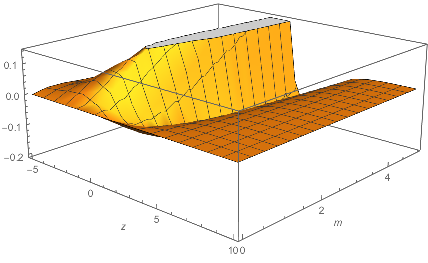
\includegraphics[scale = 0.8]{skewlogit_before_dg.png}
    \caption{$f_{1,1}(z)$ for skewed logit model, z:[-1,3], m: [0.1,3]}
    \label{fig:skewedlogit_before}
\end{figure}

% Note that $g(z)>0$, therefore we can multiply all terms by $1/g(z)$. The sequence is now $\{1/g(z), 1,z, z^2\}$. By definition of T-system and matrix algebra, we have work instead with $\{1,z, z^2,-1/g(z)\}$. 


% We will continue with 2 of \ref{proc} and add $e^z$ to the sequence.
We then add ancillary function $e^zg(z)$ to $S_1$, and divide all terms by $g(z)$. After proper permutation of order through routine algebra, we have an equivalent sequence  \{$\Psi_0(z) = 1$, $\Psi_1(z) = z$, $\Psi_2(z) = z^2$,  $\Psi_3(z) = e^z$, $\Psi_4(z) = (1+e^z)^2(-1+(1+e^{-z})^m)$\}.
% Here information matrix is expanded accordingly to  \[ \tilde{C}^*(\theta,z) = \phi(z)\left(\begin{array}{ccc}
% -(1+e^z)^2(-1+(1+e^{-z})^m) &e^z&0\\
% e^z&1 & z\\
% 0& z & z^2
% \end{array} \right).\]

We then have $f_{1,1} = 1$, $f_{2,2} =2$, $f_{3,3} = e^z/2$, 
\begin{multline*}
     -f_{4,4} = e^{-z} \left(3 (m-1) m e^{-2 z} \left(2 e^z \left(e^z+1\right)+2 e^{2 z}\right) \left(e^{-z}+1\right)^{m-2}+3 m e^{-z} \left(2 e^z \left(e^z+1\right)+2 e^{2 z}\right) \left(e^{-z}+1\right)^{m-1}-4 m e^{-z} \left(2 e^z \left(e^z+1\right)+6 e^{2 z}\right) \left(e^{-z}+1\right)^{m-1}+\left(2 e^z \left(e^z+1\right)+14 e^{2 z}\right) \left(\left(e^{-z}+1\right)^m-1\right)+6 e^{2 z} \left((m-1) m e^{-2 z} \left(e^{-z}+1\right)^{m-2}+m e^{-z} \left(e^{-z}+1\right)^{m-1}\right)+6 e^z \left(e^z+1\right) \left((m-1) m e^{-2 z} \left(e^{-z}+1\right)^{m-2}+m e^{-z} \left(e^{-z}+1\right)^{m-1}\right)+\left(e^z+1\right)^2 \left((m-3) (m-2) (m-1) m e^{-4 z} \left(e^{-z}+1\right)^{m-4}+6 (m-2) (m-1) m e^{-3 z} \left(e^{-z}+1\right)^{m-3}+7 (m-1) m e^{-2 z} \left(e^{-z}+1\right)^{m-2}+m e^{-z} \left(e^{-z}+1\right)^{m-1}\right)+8 e^z \left(e^z+1\right) \left((m-2) (m-1) m \left(-e^{-3 z}\right) \left(e^{-z}+1\right)^{m-3}-3 (m-1) m e^{-2 z} \left(e^{-z}+1\right)^{m-2}-m e^{-z} \left(e^{-z}+1\right)^{m-1}\right)\right)\\-e^{-z} \left(-3 m e^{-z} \left(2 e^z \left(e^z+1\right)+2 e^{2 z}\right) \left(e^{-z}+1\right)^{m-1}+\left(2 e^z \left(e^z+1\right)+6 e^{2 z}\right) \left(\left(e^{-z}+1\right)^m-1\right)+6 e^z \left(e^z+1\right) \left((m-1) m e^{-2 z} \left(e^{-z}+1\right)^{m-2}+m e^{-z} \left(e^{-z}+1\right)^{m-1}\right)+\left(e^z+1\right)^2 \left((m-2) (m-1) m \left(-e^{-3 z}\right) \left(e^{-z}+1\right)^{m-3}-3 (m-1) m e^{-2 z} \left(e^{-z}+1\right)^{m-2}-m e^{-z} \left(e^{-z}+1\right)^{m-1}\right)\right)
\end{multline*}

     and $F(z)<0$ for $z\in (-\infty,\infty)$. We can also visually confirm through Figure~\ref{fig:skewedlogit_after} that the surface remains below $F(z)=0$ and thus the assumptions are confirmed. Applying Theorem~\ref{2012a}, we know that considering $z\in[-A^*,B^*]$ for any large $A^*>0$ and $B^*$, the designs with at most 3 support points including $-A^*$ form a complete class. Further more, since this model is a Type III model when $m>2$ and Type I model when $m<2$, through Theorem~\ref{removepts}, there always exists a complete class of 2 support points that contains the optimal design for $m>0$. The conclusion in the following theorem follows.
     \begin{figure}[h]
    \centering
    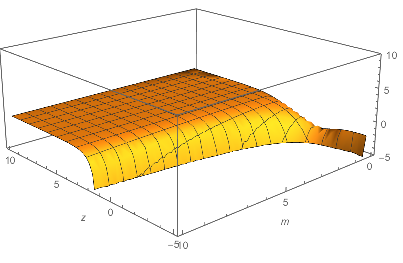
\includegraphics[scale = 0.8]{skewlogit_after_F.png}
    \caption{$F(z)$ for skewed logit model, z:[-5,10], m: [0,10]}
    \label{fig:skewedlogit_after}
\end{figure}
\begin{theorem}\label{skew}
For two parameter skewed logit model\[
P(y=1|x,\alpha,\beta) = \eta(x,\alpha,\beta)= \frac{1}{(1+e^{-\beta(x-\alpha)})^m}.
\]where $x\in (-\infty,+\infty)$. The designs with at most 2 points form a complete class.
\end{theorem}


The results of Theorem~\ref{beta}-\ref{skew} show that for Beta-Poisson model, complementary log-log model, and skewed logit model, we can find a complete class of designs with two support points that contain the optimal design regarding Loewner Ordering. Since the three models all have two parameters, the complete classes we identified were minimally supported. \cite{biedermann2006} showed the $\Phi_p$-optimal designs for these three models contain exactly two support points using the geometric approach. Our result based on Loewner Ordering provides more general results for much more optimality criteria.

    \section{Discussion}
 This paper provided an extension to the strategy in \cite{yang2010} and \cite{yang2012} to identify a complete class of designs for nonlinear models. We were able to provide resolution based on ancillary function when assumptions of Theorem~\ref{2012a} do not hold. We also showed that the added support points due to the newly added ancillary function could be removed from the final design for some models. We presented a possible procedure of doing the insertion and demonstrated with 2-parameter logistic models, Beta-Poisson model, complementary log-log model, and skewed logit model. The results are consistent with \cite{biedermann2006}. With the strategy introduced here, people will be able to identify a complete class of designs that contains the optimal design for more nonlinear models.
 
There are a few topics introduced in this paper that has yet been adequately addressed. In the models explored, we have used some shared factors of the $\Psi(z)$ functions in the sequence, but we do encourage our readers to try functions outside of the family. We do not have a full arsenal of ancillary functions yet.
% The procedure to find a proper ancillary function did not mention how exactly the insertion was selected. 

Due to the nature of optimality criterion we have chosen, we have been focusing on the Fisher information matrix which indicates the performance of least square estimator of nonlinear models. However, there are cases when parameters are estimated through other loss functions including exponential loss or Huber loss, in which case the Fisher information may not be an appropriate characterizing target. The application of the strategy for estimators through various loss functions has been explored. Extension of the information matrix in \eqref{eq:1} and \eqref{eq:2} should be explored.\


 
\nocite{*}
%\bibliographystyle{plain}
\bibliographystyle{plainnat}
\bibliography{bib_t} 
\end{document} 